\documentclass{reportClass}

\title{Torque in a Variable Reluctance Machine}
\author{G\"{o}ksenin Hande Bayazıt}
%\date{January 2019}
\universityName{Middle East Technical University}
\departmentName{Department of Electrical and Electronics Engineering}
\className{EE568 - Selected Topics on Electrical Machines}
\reportName{Project \#1 Report}

\begin{document}
\printtitle

%\tableofcontents

%\newpage

\section{Introduction}

 bıdı bıdı bıdı\\
 
 
\section{Analytical Calculations}

\par Analytical reluctance modelling of the given electromechanical system requires several assumptions on the system. Saliency of the rotor causes a change in the reluctance as the rotor rotates. Therefore, reluctance and inductance should be modelled as a function of the rotation angle, let's say $\theta$.\\

In Figure \ref{fig:angles}, some critical angles have been defined. As the rotor is in horizontally aligned position ($\theta = 0^\circ$), the air-gap is 2.5 mm. As a result, the system reluctance is maximum and the inductance is at its minimum value. When the rotation angle is $\alpha$, the air-gap becomes 0.5 mm and the reluctance starts to decrease as a function of surface area of the salient part of the rotor. When rot 

\begin{figure}[h!]
\centering
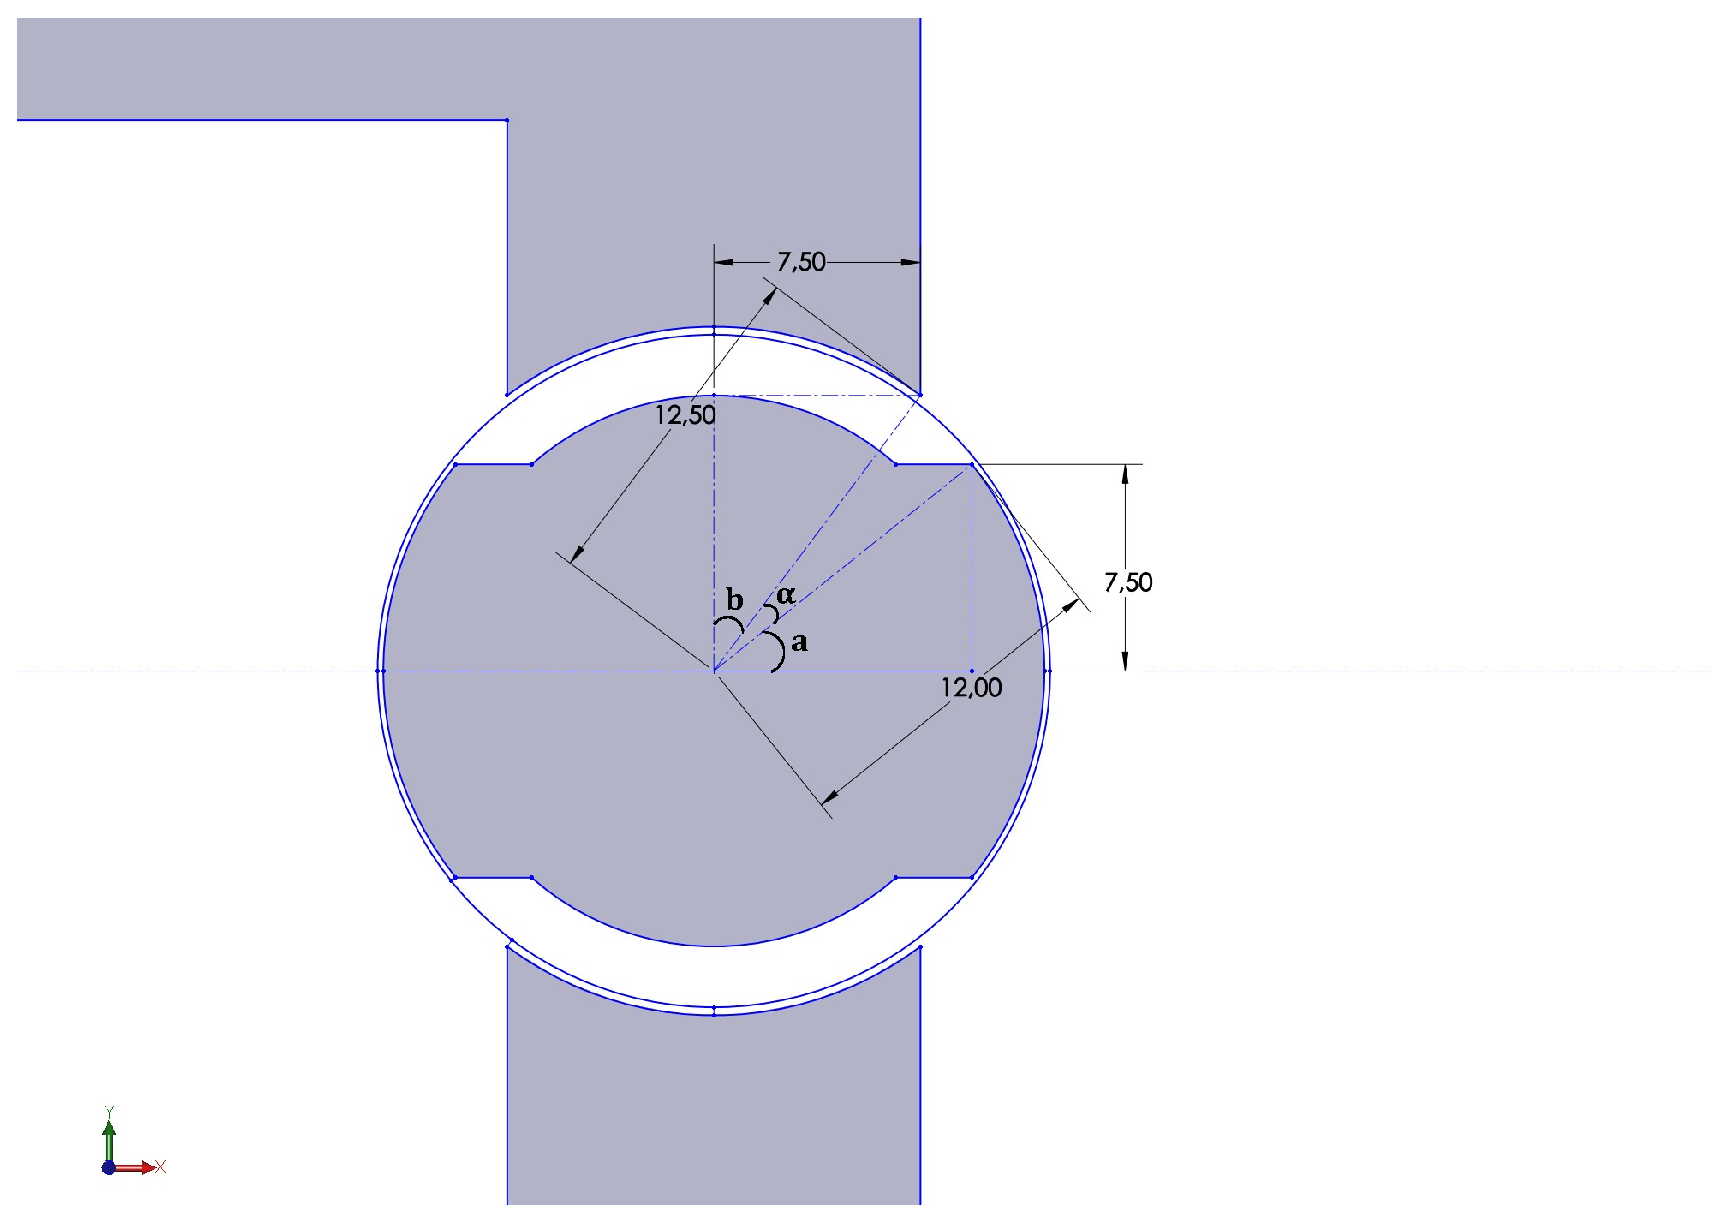
\includegraphics[trim = 40 40 140 60, clip, width=0.6\linewidth]{angles.eps}
\caption{Critical angles of the geometry for accurate reluctance modeling}
\label{fig:angles}
\end{figure}

\section{FEA Modeling (2D, Linear Material Properties)}

 bıdı bıdı bıdı

\section{FEA Modeling (2D, Nonlinear Material Properties)}

 bıdı bıdı bıdı

\section{FEA Modeling (3D, Nonlinear Material Properties)}

 bıdı bıdı bıdı

\section{Control Method}

 bıdı bıdı bıdı

\section{Conclusion}

 bıdı bıdı bıdı


\newpage

\section*{Appendix: Matlab Code for Analytical Calculations}

\input{html/analytical.tex}


\end{document}
